\chapter[量子状態]
\chapter{量子状態}


% \chaptermark{Environmental Policy Analysis with STREAM}

%\chapterauthor{Hein Mannaerts}



\begin{abstract}
Lesson abstract goes here
\end{abstract}


\section{量子ビット}
古典ビットだったら二つの状況が可能です。ビットは0か1になる。0だったらそれが100\%0だと言えます。1だったらそれが100\%1だと言えます。
% Insert qubit 100% 0
\begin{figure}[H]
    \centering
    \includegraphics[width=0.8\textwidth]{lesson2/100%0.pdf}
    \label{fig: 1}
    \begin{center}
        \caption{100\%0 キュービット}
    \end{center}
\end{figure}
量子ビットだったら\textbf{「キュービット」}と呼びますが0の状態と1の状態がありますがそれが、100\%0の状態の時もあります。その場合、この記号の中に書きます。アングルブラケット(角括弧)の中に書きます。
% Insert qubit 100% 1 
\begin{figure}[H]
    \centering
    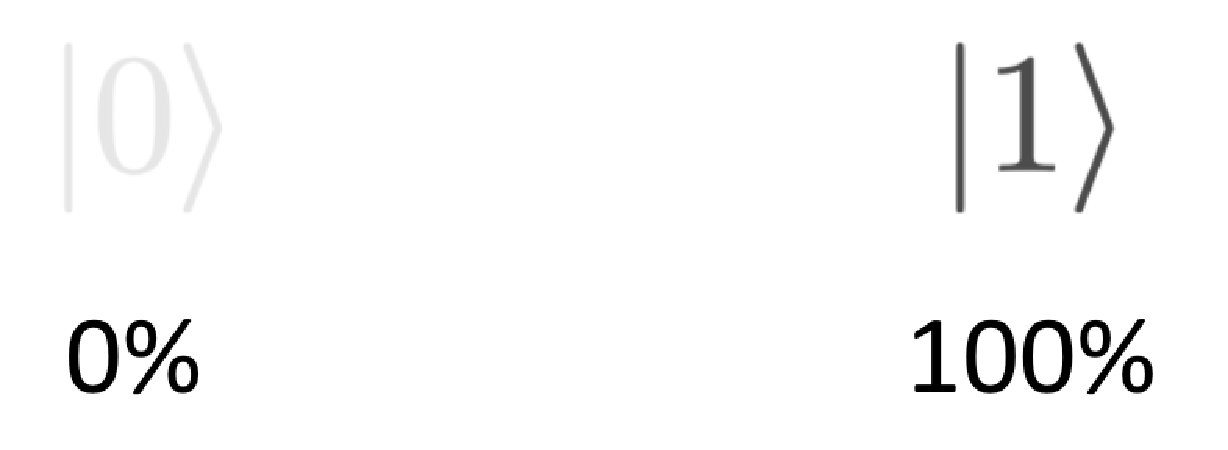
\includegraphics[width=0.8\textwidth]{lesson2/100_1.pdf}
    \label{fig: 1}
    \begin{center}
        \caption{100\%1 キュービット}
    \end{center}
\end{figure}
もし1の状態だったら1をアングルブラケットの中に書きます。100\%1の状態の時に
ですが、それだけじゃなく\emph{その間の状態}も可能です。
% Insert superposition state pic.
\begin{figure}[H]
    \centering
    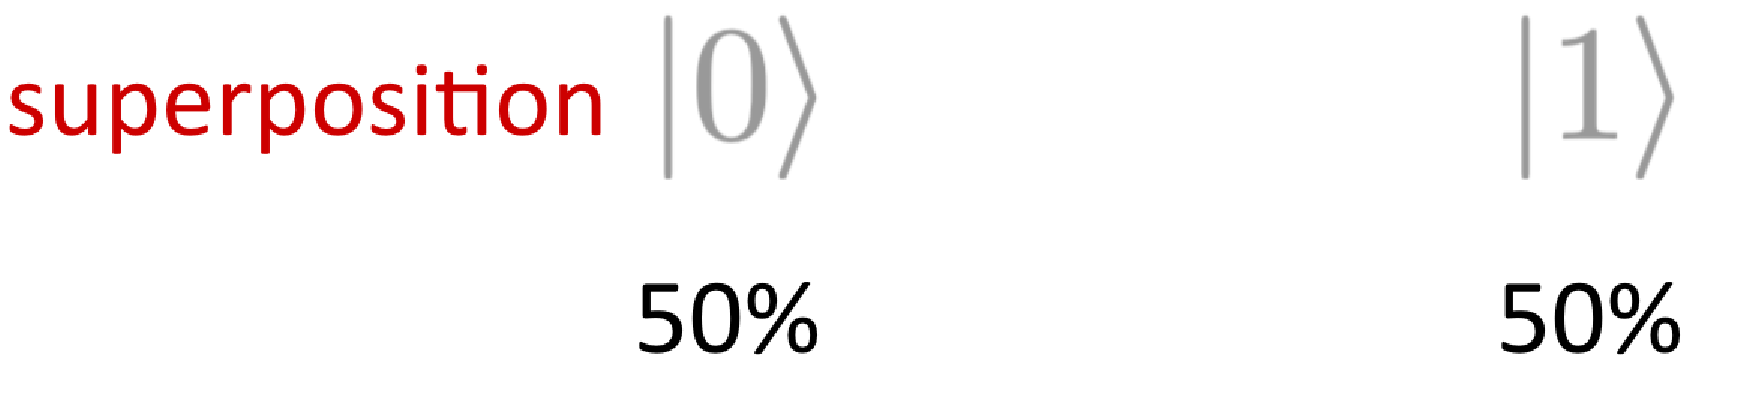
\includegraphics[width=0.8\textwidth]{lesson2/superposition_qubit.pdf}
    \label{fig: 1}
    \begin{center}
        \caption{重ね合わせ状態キュービット}
    \end{center}
\end{figure}
例えば50\%0の状態プラス50\%1の状態。その場合、この様に書きます。これを\textbf{重ね合わせ}と言います。この重ね合わせの状況は古典のビットにはできないですよね。
この記号この書き方をもう少し説明しましょう。
\begin{equation}
\ket{\psi} = \alpha \ket{0} + \beta\ket{1} 
\end{equation}
これは、\textbf{ディラックノーテーション}と言います。この左側に書いてある状態は$\psi$ (\emph{psi}) の状態と言いますが、(\emph{alpha}) かける0プラス\emph{beta}かける1と読みます。
% Dirac Notation w/ annotation
\begin{figure}[H]
    \centering
    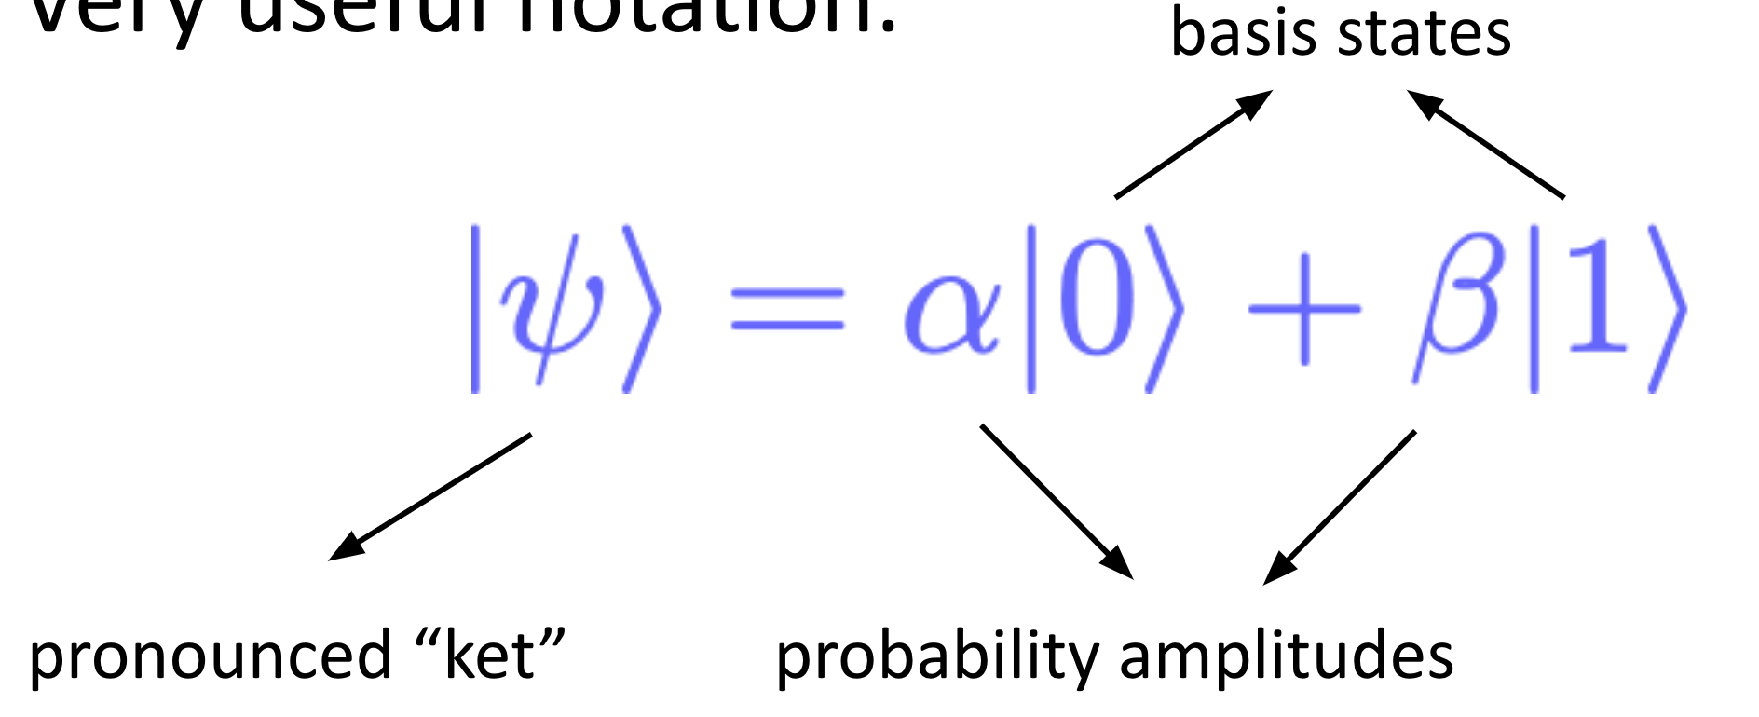
\includegraphics[width=0.8\textwidth]{lesson2/dirac_notation.pdf}
    \label{fig: 1}
    \begin{center}
        \caption{ディラックノーテーション}
    \end{center}
\end{figure}
$\psi$, 0, 1 を囲むのは\textbf{ケットノーテーション}と言います。これがケット記号。この0と1は\textbf{basis state}、つまり基底ベクトルです。この$\alpha$と$\beta$は\textbf{probability amplitudes}、つまり、確率振幅です。 これは複素数になることが可能です。これは正規化しなければならになりませんので、絶対$\alpha$の二乗足す絶対$\beta$ の二乗 が1に等しくなければなりません。
% Bloch Sphere
\begin{figure}[H]
    \centering
    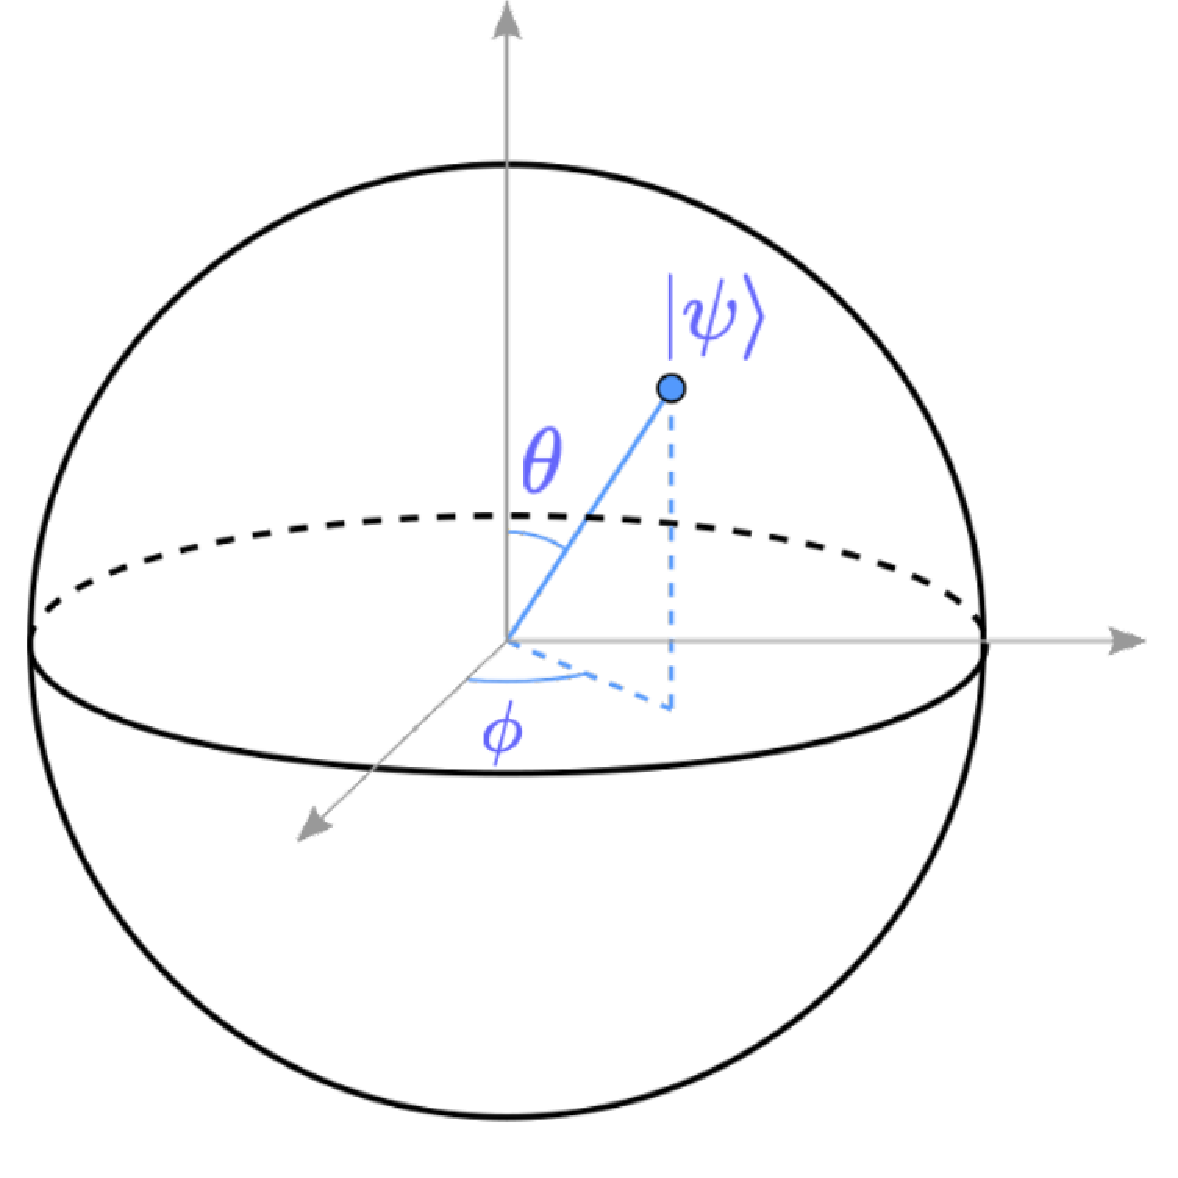
\includegraphics[width=0.6\textwidth]{lesson2/bloch_sphere.pdf}
    \label{fig: 1}
    \begin{center}
        \caption{ブロッホ球}
    \end{center}
\end{figure}
もう一つの表示の仕方としては\textbf{ブロッホ球}があります。このブロッホ球は1つの量子ビットの状態を表示できます。これは2つの角度を使うんですが、
$\theta$の角度と$\phi$の角度でこの$\psi$の状態を書きます。そうするとこの$\psi$の状態は次のように表せます。
\begin{equation}
|\psi\rangle=\cos \frac{\theta}{2}|0\rangle+e^{i \phi} \sin \frac{\theta}{2}|1\rangle
\end{equation}

この$e^{i\phi}$は\textbf{phase}、あるいは位相と言います。これは一つの量子ビットは二つの角度で定義できますがもう一つの言い方をすると三次元の球なのでX軸、Y軸、Z軸を使います。
% insert Bloch sphere w/ axes labelled and |+> |-> meanings
\begin{figure}[H]
    \centering
    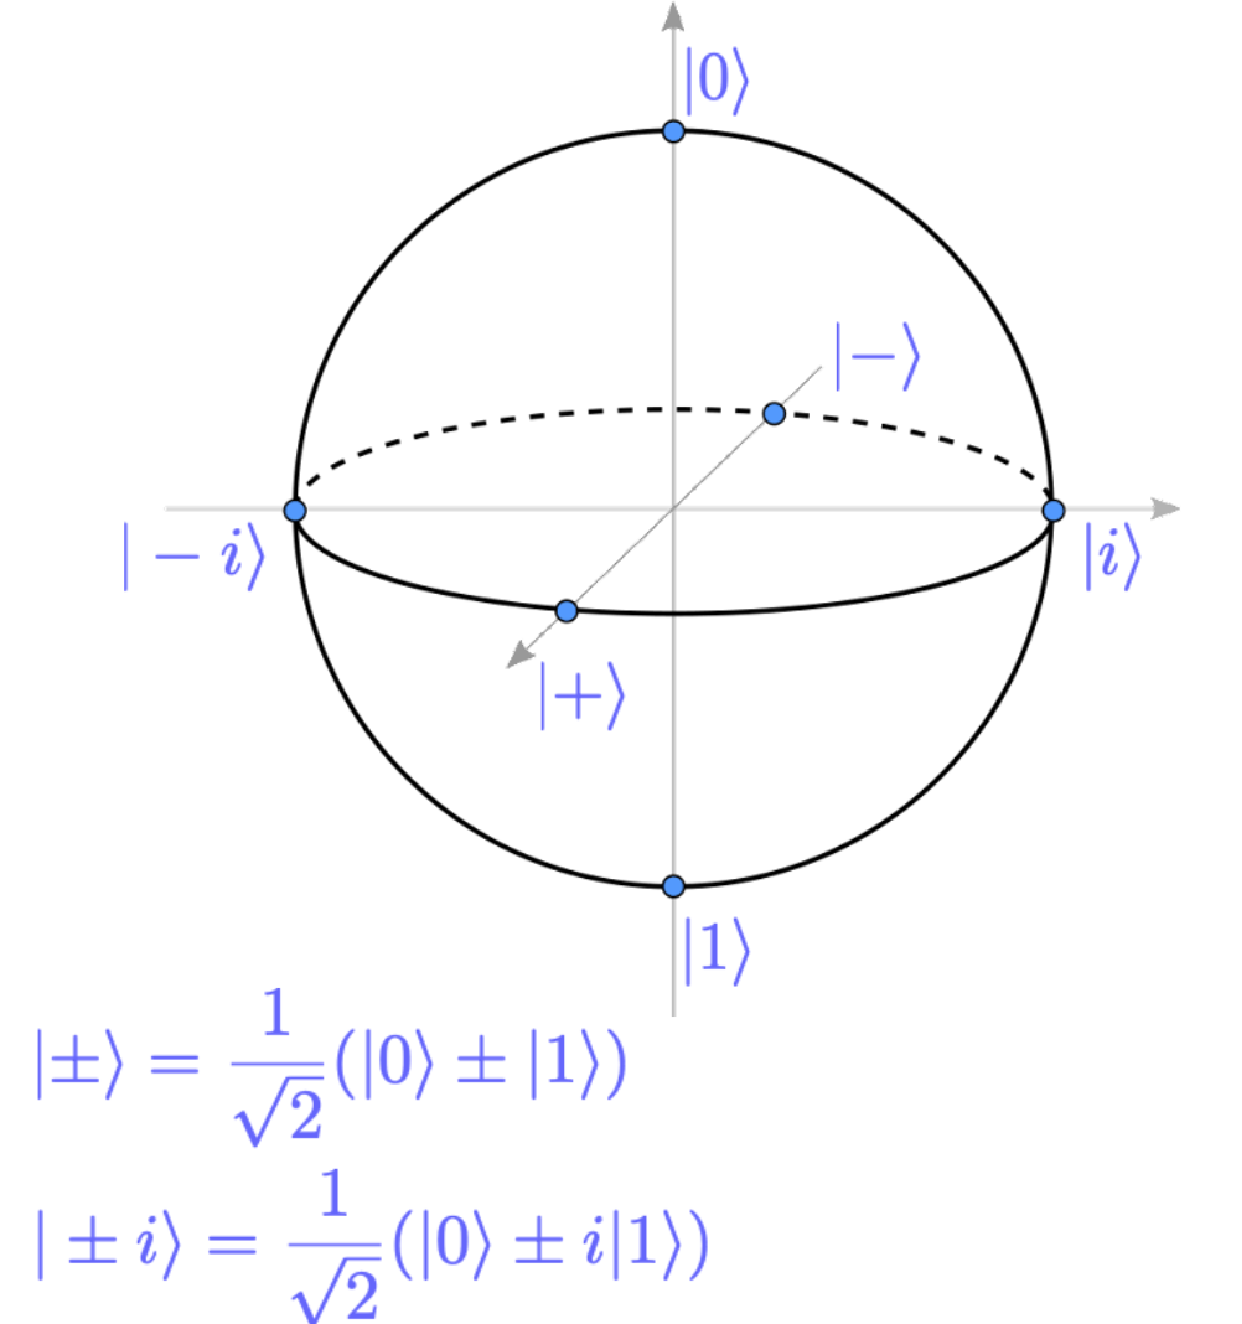
\includegraphics[width=0.7\textwidth]{lesson2/bloch_sphere_annotated.pdf}
    \label{fig: 1}
    \begin{center}
        \caption{ブロッホ球 軸解説}
    \end{center}
\end{figure}
このZ軸は縦の所で0の状態はブロッホ球の一番上の所。1の状態はブロッホ球の一番下の所にあります。そうすると、X軸は赤道にありますがその赤道は前と後ろの方に別れています。前の方の所を+( プラス)の状態と言います。後ろの所を-(マイナス)の状態と言います。なぜこれが+と-の状態と言うのかはこういう風に書くから。0と1じゃなくてこのket notationの中には+と-のを書きます。そうするとこれは、0+1の状態。あるいは0-1の状態になりますすると正規化しなければなりませんので$\sqrt{\frac{1}{2}}$をかけます。そうすると正規化できるでしょう。

続いて、Yの軸の場合+iと-iと言います。それがさっきの所の$\phi$の角度でこれは位相が変更されます。状態を書きますと、さっきと同じ+と-の状態で0+1のなんですけど、間は0と+だけじゃなくて、かけるiになります。これはさっきの位相です。
そうすると、これが+-iの状態で、それがY軸の右と左の所になります。これは一つの量子ビットだけなんで複数の量子ビットには使えない表示の仕方です。


\section{ユニタリ演算}
情報を処理すると何かの物理的なシステムを使います。
% Classical (SSD) VS Quantum (Ion Trap)
\begin{figure}[H]
    \centering
    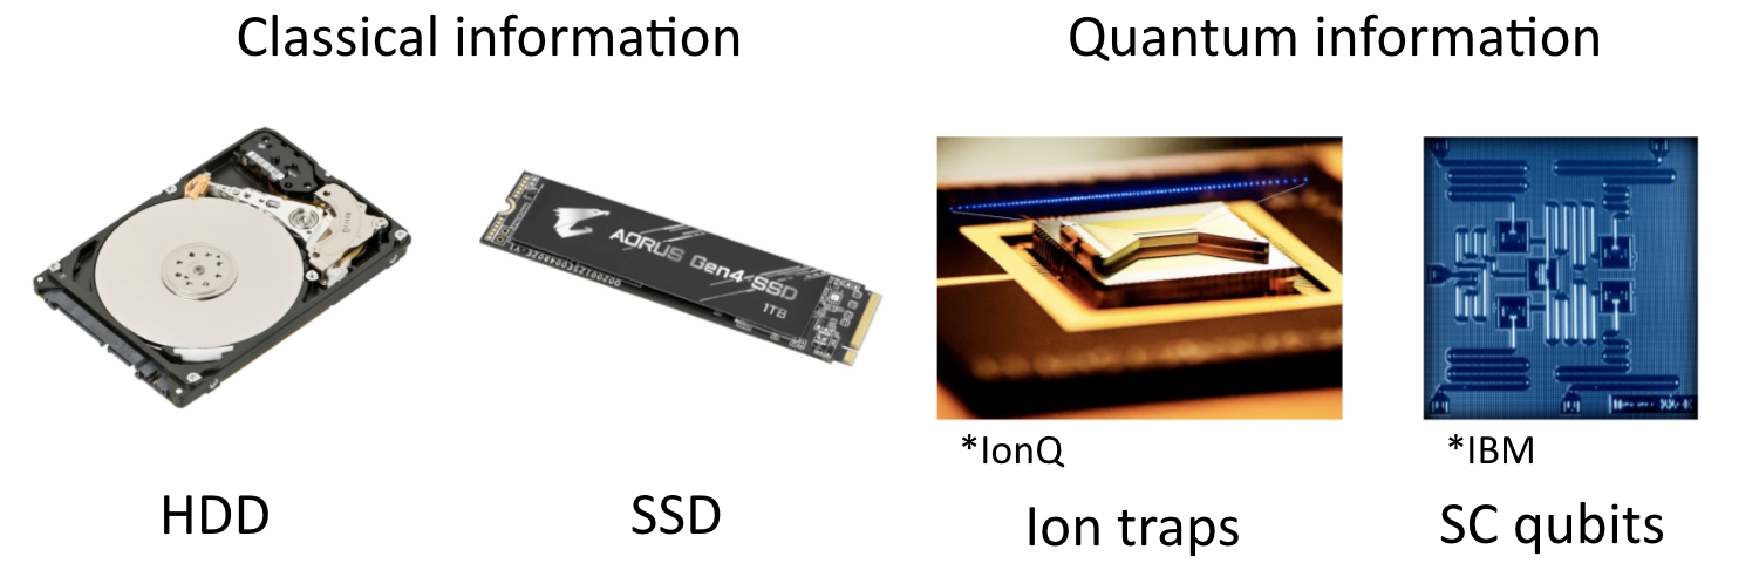
\includegraphics[width=0.7\textwidth]{lesson2/ion_trap_etc.pdf}
    \label{fig: 1}
    \begin{center}
        \caption{物理的なシステム}
    \end{center}
\end{figure}
それは例えば物理のシステムを相互作用しなければなりませんが例えば古典の場合だったら磁気ディスクにデータを保存することも可能性ですしSolid State Driveにもデータを保存することが可能です。これが物理的にはビットの効果で出来ているんですが量子の場合だったら量子情報は例えばこの左側の真ん中のところには
イオントラップがあります。このイオントラップの中にはチップ型の物の上に原子が一個ずつ浮かびます。原子が量子ビットを表示する。その量子ビットを作用すると
計算ができる様になります。例えば右側のは超伝導のチップ、これはIBMの例なんですが、これも量子伝導という量子効果を使ってこれに量子作用による量子影響が起こるとこれが
データを表示してデータを処理できる様になります。これを数学的にも見てみましょう。
\subsection{いくつかの演算}
% Simple Unitary Operations 
\begin{figure}[H]
    \centering
    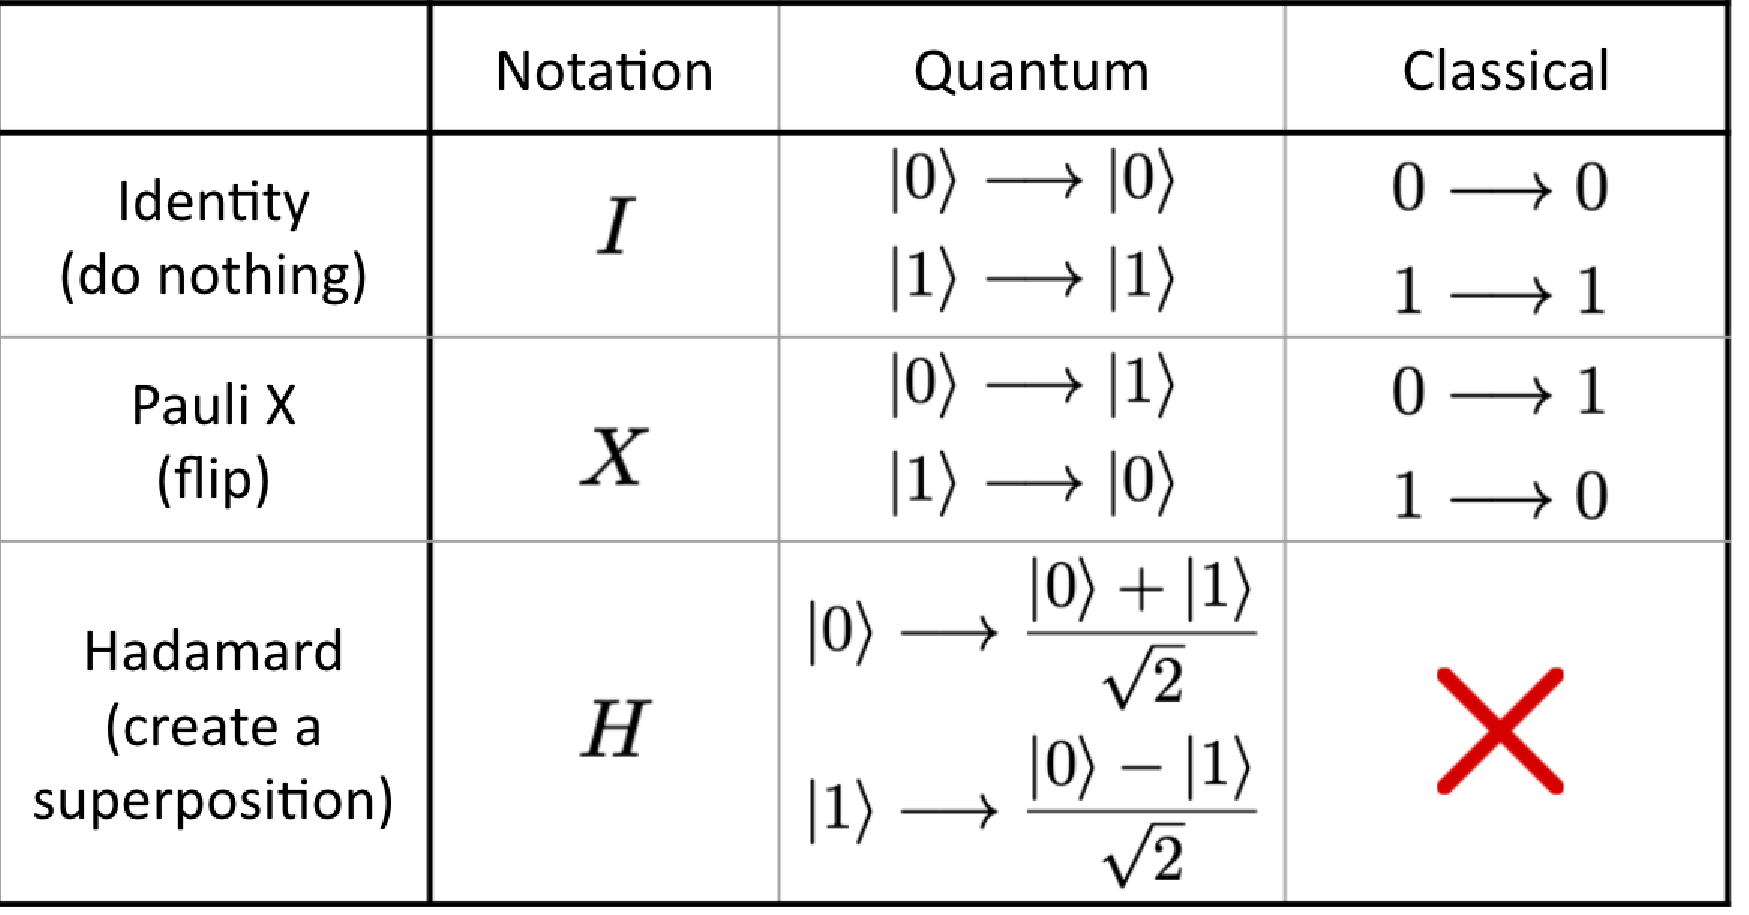
\includegraphics[width=0.7\textwidth]{lesson2/simple_unitary_ops.pdf}
    \label{fig: 1}
    \begin{center}
        \caption{シンプルユニたり演算}
    \end{center}
\end{figure}
まずはこれをユニタリ演算と言いますが例えば一番最初に学ぶのはI(アイデンティティ行列)。このアイデンティティ行列は単位行列です。右側の所には古典(classical)のデータの処理がIdentity Matrixを通ると0のinput stateはそのまま0になり1のinput stateもそのまま1になります。量子の場合だったら一緒で0の状態をinputしたら0の状態がoutputされます。1の状態をinputしたら1の状態がoutputされます。つまり、何も計算せず何も変わらない。これをデータ保存とも言える。

もう一つの例としてパウリ行列のXがありますXの場合は大文字のXで書く。これが\textbf{パウリXユニタリ演算}と言います。これがbit flipになりますそのbit flipというのは古典の場合0が1になり1が0になる。古典の場合これをNotとも言う。
量子の状態でも0の状態をinputしたら1の状態が出てきます。1の状態を入れたら0の状態が出てきます。これも一緒でNotとも言えますが量子の場合だとXゲートあるいはX演算と言います。

もう一つの例として\textbf{Hadamardゲート}があります。Hadamard演算ですがこれは大文字のHを書きます。Hの他の使い方もありますがここではHadamardという意味ですね。Hの場合inputが0だった時outputは0足す1の重ね合わせこれがさっきのステップで言っていた様に正規化もしなければいけないので割る$1/\sqrt{2}$にします。
1のinputをしたら1と0の重ね合わせの結果が出てくる。このoutputの場合位相も違い+ではなく-になる。これも正規化するために割る√2しなければならない。このゲートがこのユニタリ演算は重ね合わせを作る基本の演算となります。この場合古典のデータだと重ね合わせというのはないので古典の場合ありません。
\subsection{ユニたり演算}
さて先程はユニタリ演算という言葉を使っていましたがユニタリ演算て何でしょう?
まあユニタリ演算というのは逆計算が可能な演算です。その逆計算を\textbf{adjoint}と言います。adjointと言うのは随伴です.書くとUが最初の演算だったら$U^{\dagger}$と記号、dagger(短剣符)を使って随伴と言う。そうするとinput stateは$\psi$のケットの場合$U$の演算を掛けると$\psi^\prime$の結果が出て$U^{\dagger}$を掛けると$\psi$の状態に戻る。これは逆計算が可能になっているでしょう。
最初は$\psi$の状況だったが何かを計算し変更されてもう一回やることでoutputと
inputの状態が同じになったので逆計算ができ、これが随伴この$\psi^\prime$という状態が$U$掛ける最初のinputの$\psi$のstateで、$\psi$も$U^{\dagger}$掛ける$\psi^\prime$の状態になるんです。

ちょっと数学的にやってみると$\psi$の状態を
\begin{equation}
|\psi\rangle=U^{\dagger}\left|\psi^{\prime}\right\rangle=U^{\dagger} U|\psi\rangle
\end{equation} 
これは最初の$\psi$と最後の$\psi$が等しくなるためにはこの$U^{\dagger} U$は$I$(アイデンティティ行列)にしなければならない。もう一つの計算手法としては$\psi^{\prime}$にすると
\begin{equation}
\left|\psi^{\prime}\right\rangle=U|\psi\rangle=U U^{\dagger}\left|\psi^{\prime}\right\rangle
\end{equation}
これは最初の$\psi^{\prime}$と最後の$\psi^{\prime}$が等しくなるために$UU^{\dagger} = I$ なので
\begin{equation}
U U^{\dagger}=U^{\dagger} U=I
\end{equation}
でこれはこの演算も行列なのでこれは随伴行列と言います。(adjoint operator, adjoint matrix)。
\subsection{行列表示}
もう少し行列の話をすると状態をベクトルで表示することができますがユニタリ演算は行列で表示します。例えば状態をちょっと見てみましょう。0の状態を古典と同じ様に0と1を使ってるんですが量子の0の状態を使うとこれが本当は
\begin{equation}
|0\rangle=\left(\begin{array}{l}
1 \\
0
\end{array}\right)
\end{equation}
ベクトルとしては$1, 0$の二次元の状態となる。1の状態だったらこれも同様に
\begin{equation}
|1\rangle=\left(\begin{array}{l}
0 \\
1
\end{array}\right)
\end{equation}
二次元のベクトルで1, 0じゃなくて0, 1になります。そして、一つの量子ビットの状態を表示するためには$\psi$と言いますが
\begin{equation}
|\psi\rangle=\alpha\left(\begin{array}{l}
1 \\
0
\end{array}\right)+\beta\left(\begin{array}{l}
0 \\
1
\end{array}\right)=\left(\begin{array}{l}
\alpha \\
\beta
\end{array}\right)
\end{equation}になりますね。

これもベクトルで1つの量子ビットの状態を表示できる様になる。後で$\psi$の変数としては色んな使い方で使いますが今の場合は1量子ビットだけです。

するとさっき言ってたIのoperatorが行列で書かなければけませんが

0:09:00.483,0:09:05.411
これは
\begin{equation}
I=\left(\begin{array}{ll}
1 & 0 \\
0 & 1
\end{array}\right)
\end{equation}
の行列で斜めの所は全て1なので\textbf{diagonal, diagonal}じゃない所は全部0になる行列になります。これは2掛ける2の行列ですがもっと大きいやつもできます。それとこれからよく使う行列は三つあります。
さっきはパウリ行列のXの例を見せたんですが
三つもありますね\textbf{X}と\textbf{Y}と\textbf{Z}. \textbf{Pauli operator}、パウリ行列と言います。
\begin{equation}
\begin{aligned}
&X=\left(\begin{array}{ll}
0 & 1 \\
1 & 0
\end{array}\right) \\
&Y=\left(\begin{array}{cc}
0 & -i \\
i & 0
\end{array}\right) \\
&Z=\left(\begin{array}{cc}
1 & 0 \\
0 & -1
\end{array}\right)
\end{aligned}
\end{equation}
この場合もう少し説明するとブロッホ球にも便利な考え方をできるので後で見せます。Hadamard の行列だったらこれはHで書くんです。
\begin{equation}
H=\frac{1}{\sqrt{2}}\left(\begin{array}{cc}
1 & 1 \\
1 & -1
\end{array}\right)
\end{equation}
\subsection{演算作用}
さてこの演算はどの様に作用するのか?まずはXの行列を見てみましょう。これはbit flipと言っていたんですが:
\begin{equation}
\begin{aligned}
X|0\rangle &=\left(\begin{array}{ll}
0 & 1 \\
1 & 0
\end{array}\right)\left(\begin{array}{l}
1 \\
0
\end{array}\right) \\
&=\left(\begin{array}{l}
0 \\
1
\end{array}\right)=|1\rangle
\end{aligned}
\end{equation}
縦のベクトルと線形代数の授業で学んだ行列の掛け算をすると出てくるベクトルは1の状態です。逆の方にするとXの状態掛ける1の状態だったら:
\begin{equation}
\begin{aligned}
X|1\rangle &=\left(\begin{array}{ll}
0 & 1 \\
1 & 0
\end{array}\right)\left(\begin{array}{l}
0 \\
1
\end{array}\right) \\
&=\left(\begin{array}{l}
1 \\
0
\end{array}\right)=|0\rangle
\end{aligned}
\end{equation}
0の状態が出てきます。次は重ね合わせを作りたいです。この重ね合わせを作りたい場合はHadamard演算を使いますが
これはH掛ける0の状態だったら:
\begin{equation}
\begin{aligned}
H|0\rangle &=\frac{1}{\sqrt{2}}\left(\begin{array}{cc}
1 & 1 \\
1 & -1
\end{array}\right)\left(\begin{array}{l}
1 \\
0
\end{array}\right) \\
&=\frac{1}{\sqrt{2}}\left(\begin{array}{l}
1 \\
1
\end{array}\right)=\frac{1}{\sqrt{2}}(|0\rangle+|1\rangle)
\end{aligned}
\end{equation}

% 計算通り出てくる状態が0+1掛ける√1/2

するとH掛ける1の状態だと算数は一緒なんですが:
\begin{equation}
\begin{aligned}
H|1\rangle &=\frac{1}{\sqrt{2}}\left(\begin{array}{cc}
1 & 1 \\
1 & -1
\end{array}\right)\left(\begin{array}{l}
0 \\
1
\end{array}\right) \\
&=\frac{1}{\sqrt{2}}\left(\begin{array}{c}
1 \\
-1
\end{array}\right)=\frac{1}{\sqrt{2}}(|0\rangle-|1\rangle)
\end{aligned}
\end{equation}


二つとも重ね合わせを作っていますが一つはプラスの状態ともう一つはマイナスの状態になりますね。そうする二つの重ね合わせの作り方があり、一つはが違う
マイナスの状態だったら位相は掛けるπになっている。
\subsection{随伴行列}
さて、随伴行列とさっき言ってと思うんですが随伴行列というのはどの様に作ることができるのでしょう?まずは一つの複素数で\textbf{complex conjugate}を作らなければならない。complex congutateというのは複素共役ですね。これも線形代数または高校で学んだことだと思うんですけど
\begin{equation}
(x+i y)^{*}=x-i y
\end{equation}
この(*)の星のマーク、星のマークをつけるとそれが共役という意味なんですが$i$の所はプラスがマイナスになる。上に示されているようになります。
もう一つのやらなければいけないことが、もし最初のUが2x2の行列だったら:
\begin{equation}
U=\left(\begin{array}{ll}
U_{00} & U_{01} \\
U_{10} & U_{11}
\end{array}\right) \rightarrow\left(\begin{array}{cc}
U_{00}^{*} & U_{01}^{*} \\
U_{10}^{*} & U_{11}^{*}
\end{array}\right) \longrightarrow\left(\begin{array}{ll}
U_{00}^{*} & U_{10}^{*} \\
U_{01}^{*} & U_{11}^{*}
\end{array}\right)=U^{\dagger}
\end{equation}
$U_{00}$, $U_{01}$, $U_{10}$, $U_{11}$ なんですがそれの位置を変更します。
これが転置行列になるんですが、diagonalの所は変わりませんがoff diagonalの位置がswapすることになります。斜めが45度の角度みたいな所は行列をflipする
となるとこれが$U^{\dagger}$ の状態になりますね。\textbf{式1.17}の風に書きます。これがそうすると随伴行列を作るために複素数共役と斜めにflipするとこのadjoint matrixができます。例としてパウリのY行列を見てみましょう :
\begin{equation}
Y=\left(\begin{array}{cc}
0 & -i \\
i & 0
\end{array}\right) \longrightarrow\left(\begin{array}{cc}
0 & i \\
-i & 0
\end{array}\right) \longrightarrow\left(\begin{array}{cc}
0 & -i \\
i & 0
\end{array}\right)=Y
\end{equation}
このパウリのY行列が\textbf{式1.10}で見せたようの2x2の行列です。まず共役にし、行列をflipすると出てくるものは元の状態と一緒、つまり
$Y$のadjoint matrixが $Y$。こういう場合\textbf{self adjoint matrix }あるいは自己随伴行列。
\subsection{回転}
そして重要なユニタリ演算の種類が回転と言えるんですが。

これが数式をみると抽象的なことなんですが:
\begin{equation}
R_{\hat{n}}(\theta)=e^{-i \theta \hat{n} \cdot \hat{\sigma} / 2}
\end{equation}
になりますね。ちょっと複雑な表現でしょう。まあこの場合だったら$\hat{n}$はベクトルなんですけれども、$\hat{n} = (n_x, n_y, n_z)$で$\hat{\sigma}$ は\textbf{式1.10}からの行列で、 $\hat{\sigma} = (X,Y,Z)$になります。
まあそれがこの$e$の何乗かを計算するとこの様な表示が出てきます:
\begin{equation}
e^{-i \theta \hat{n} \cdot \hat{\sigma} / 2 }=\cos \frac{\theta}{2} I-i \sin \frac{\theta}{2}\left(n_{x} X+n_{y} Y+n_{z} Z\right)
\end{equation}
まあちょっと複雑なんですが。

もうちょっと簡単な考え方にすると先程紹介したブロッホ球が使えます。
% insert Bloch sphere rotation y-axis
\begin{figure}[H]
    \centering
    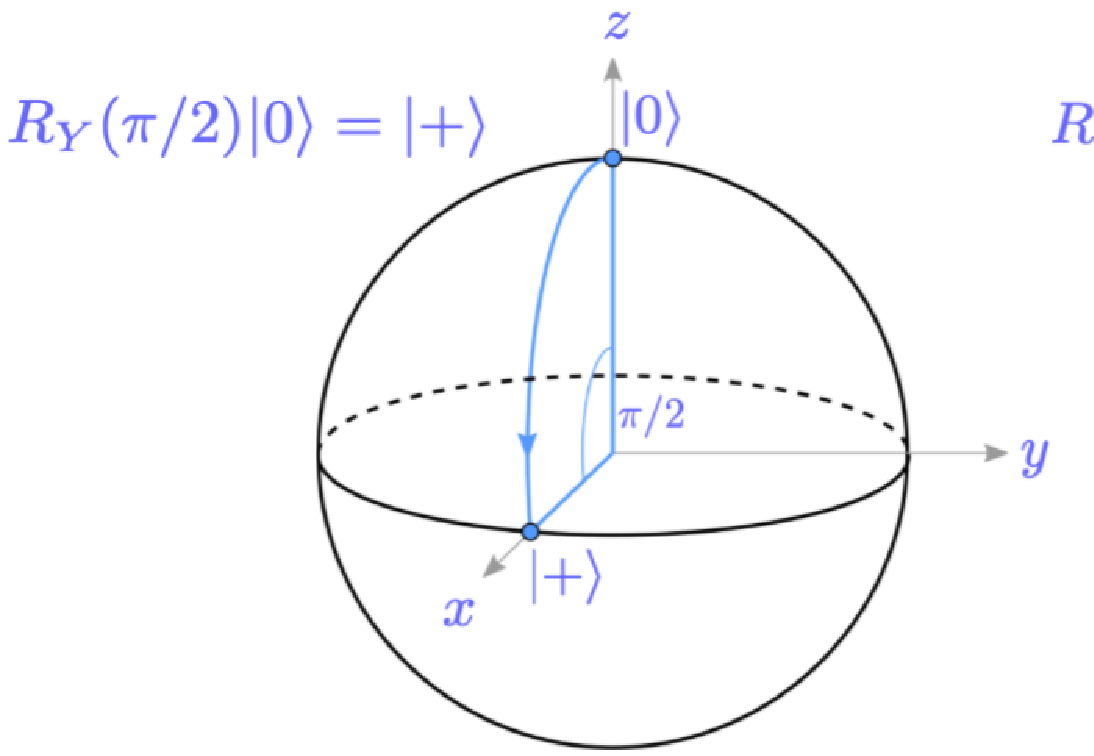
\includegraphics[width=0.7\textwidth]{lesson2/bloch_y_axis.pdf}
    \label{fig: 1}
    \begin{center}
        \caption{Y軸回転}
    \end{center}
\end{figure}
例えばこれがY軸を回転したい場合するとこのY軸はこの場合左右にありますが、まずはinput stateを0にするとこの場合
$\pi/2$の$Y$の回転にすると
\begin{equation}
R_{Y}(\pi / 2)|0\rangle=|+\rangle
\end{equation}
プラスの状態というのはこの角度を$\pi/2$回転するでしょう。で北極の所から赤道まで下がる。するとこれがX軸のてっぺんの所の+になります。まあこれだけじゃなく色んな場所で回転は可能です。
\begin{figure}[H]
    \centering
    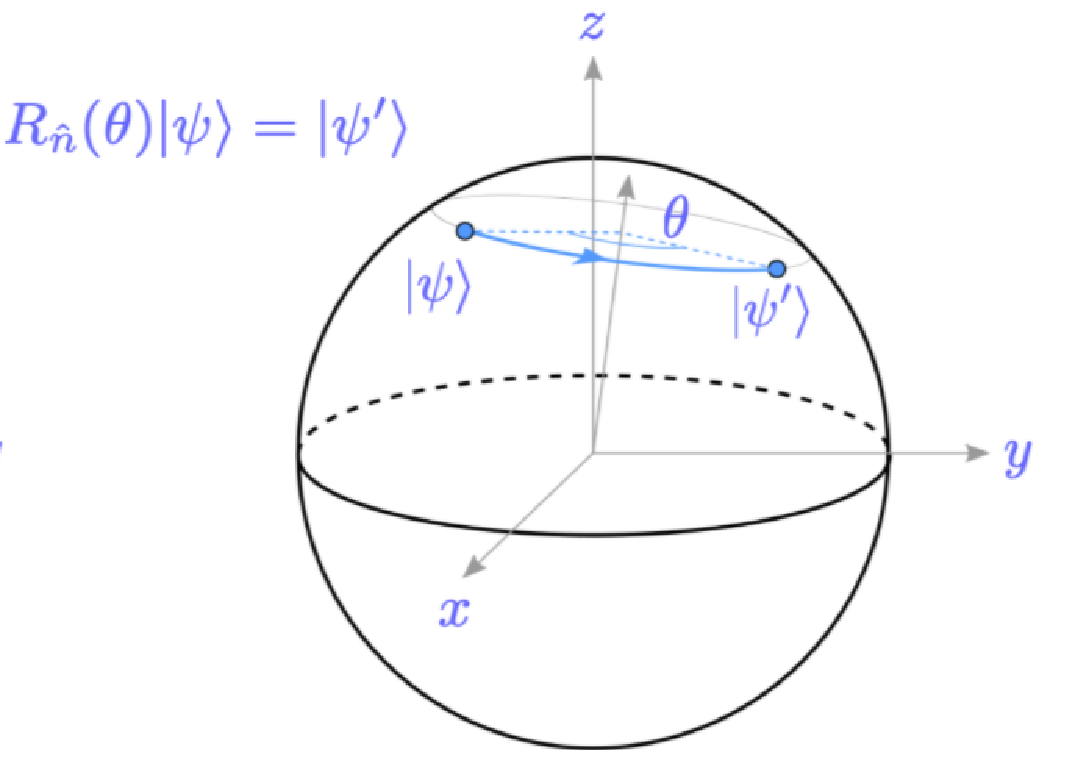
\includegraphics[width=0.7\textwidth]{lesson2/bloch_general_axis.pdf}
    \label{fig: 1}
    \begin{center}
        \caption{任意軸回転}
    \end{center}
\end{figure}
この場合斜めのベクトルを軸としてこの上で回転したいので$\psi$の状態を$\psi^\prime$に回転することがこれがさっきの汎用の所の
\begin{equation}
R_{\hat{n}}(\theta)|\psi\rangle=\left|\psi^{\prime}\right\rangle
\end{equation}
これがユニタリ演算の基礎の数学です。

\section{測定}
測定の目標としてはシステムから情報を読み出す。読み出しが量子のデータから古典のデータになるんですけれども、例えば一番知りたい事はこの量子ビットが0の状態か1の状態かどっちですか?その質問を答えたいです。
\subsection{パウリZ軸測定}
\begin{figure}[H]
    \centering
    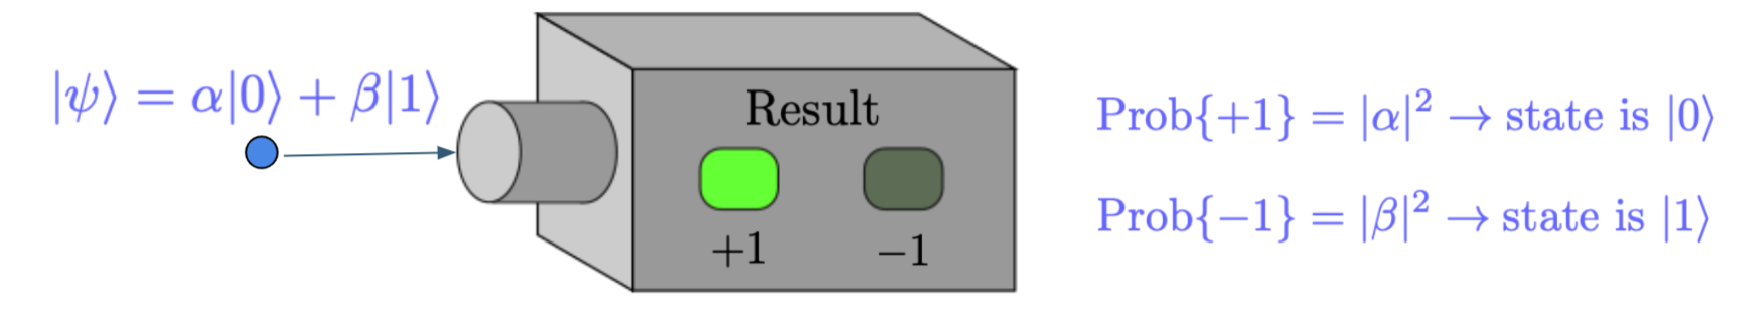
\includegraphics[width=0.7\textwidth]{lesson2/Pauli_z_machine.pdf}
    \label{fig: 1}
    \begin{center}
        \caption{Z軸測定}
    \end{center}
\end{figure}
じゃあ例えばこれが機械になるんですけれどもinputとしては何か知らない量子ビットの状態を入れるんですがこの装置に入れて出てくる結果が$+1$か$-1$が出てきます。

その$+1$か$-1$だったらまあこの場合その最初のインプットの$\psi$のstateが
\begin{equation}
|\psi\rangle=\alpha|0\rangle+\beta|1\rangle
\end{equation}
の状態だったらその$+1$出てくる確率が絶対$|\alpha|^{2}$で$-1$が出てくる確率が絶対$|\beta|^{2}$
そうするとこれが \textbf{Quantum measurement}の基礎です。この場合だったらパウリのZ軸で測定するんですけれどもさっきのブロッホ球の所にはこれがブロッホ球の一番上か下になる事なんですね。これは \textbf{computational basis}と言いますけれどもそれが計算基底ですね。
\subsection{パウリX軸測定}

まあもう一つの測定の仕方があるんですけれども、この状況は0状態が0ですか1ですかじゃなくてこの状態が+ですか-ですかとの質問も問うことが可能でしょう。
すると線形代数を使うと:
\begin{equation}
|0\rangle=\frac{1}{\sqrt{2}}(|+\rangle+|-\rangle) \quad|1\rangle=\frac{1}{\sqrt{2}}(|+\rangle-|-\rangle)
\end{equation}
と表示できます。1の状態だったらマイナスの状態には位相をつけるでしょう。
\begin{figure}[H]
    \centering
    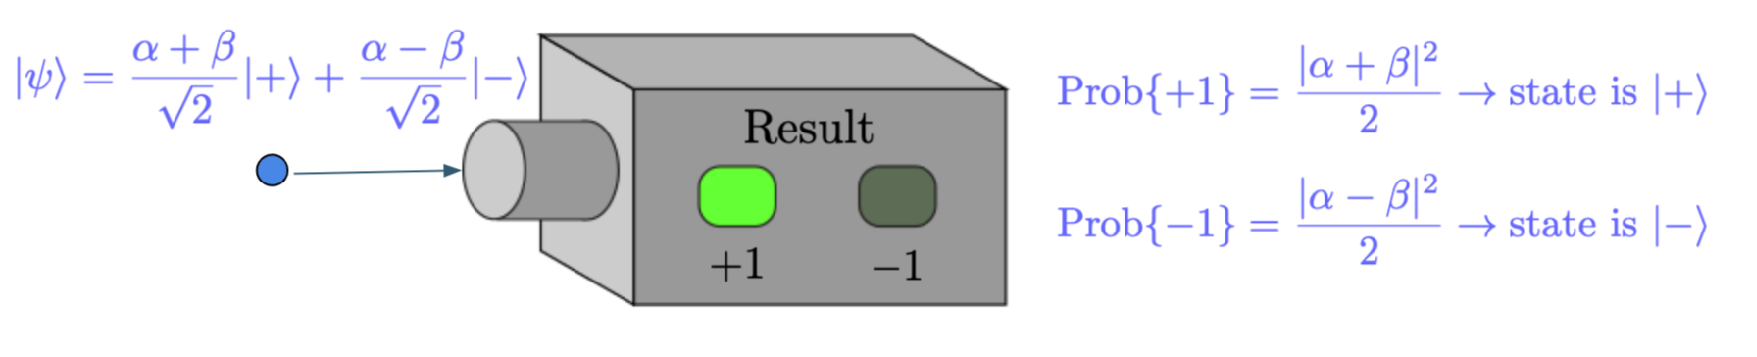
\includegraphics[width=0.7\textwidth]{lesson2/Pauli_x_machine.pdf}
    \label{fig: 1}
    \begin{center}
        \caption{X軸測定}
    \end{center}
\end{figure}
そうするとこの状態を入れると:
\begin{equation}
|\psi\rangle=\frac{\alpha+\beta}{\sqrt{2}}|+\rangle+\frac{\alpha-\beta}{\sqrt{2}}|-\rangle
\end{equation}
そうすると$+1$が出てくる確率が$\alpha +\beta$の絶対値とそれの二乗割る2、-1が出てくる確率が$\alpha-\beta$の絶対値二乗割る2。そうするとこれがが$+$になってくる確立と$-$で出てくる確率はそれも表示できます。
これは\textbf{Pauli X Basis}、\textbf{Figure 1.10}のブロッホ球のところに$+$がX軸のブロッホ球の赤道のところには X軸の一番手前のところと$-$が一番後ろでしょう。そうするとこれがその状態として表示できます。
\subsection{線形代数}
さてこれは基底と言ってるんですけれども$0$, $1$の基底あるいは$+$,$-$の基底と言います。線形代数の授業で学んだと思うんですけれども\textbf{basis set}このbasis setというのは基底setなんですがそれがベクトルどんなベクトルも表示できるベクトルのセットと言える。2次元の紙だったらX軸+Y軸だったらなんでもその紙の上のところになんでも定義できるでしょう。

まあこの場合だったら$\psi$の状態を表示しているんですけどもこれは\textbf{Pauli Z basis} が0の状態と1の状態。この2つはまあ一つの量子ビットで二次元のシステムなんですけれどもその0と1が基底セットになる。
% Insert basis representation pic here.
\begin{figure}[H]
    \centering
    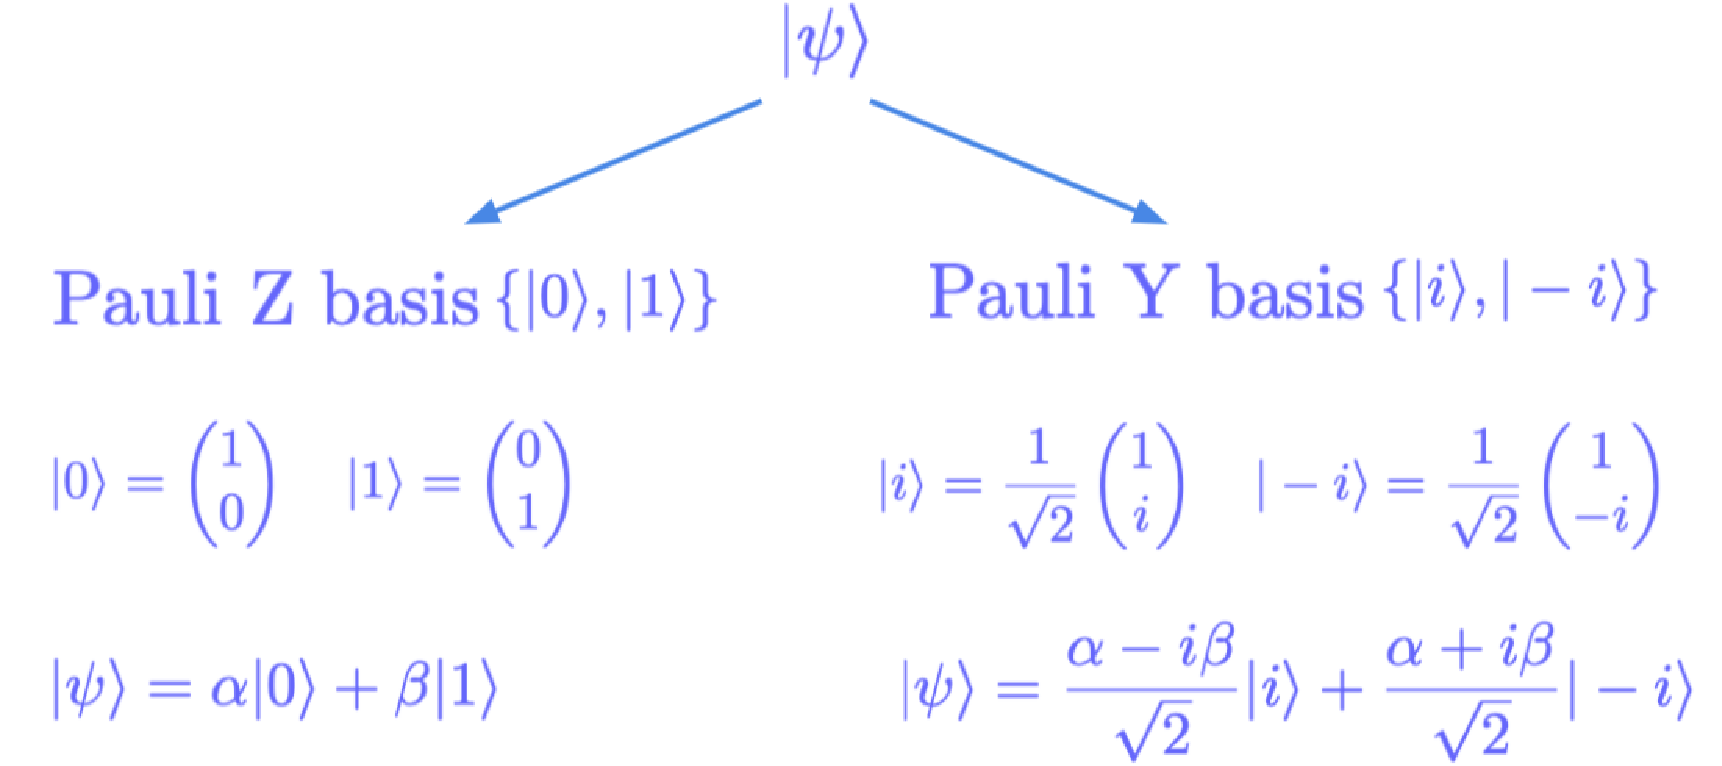
\includegraphics[width=0.7\textwidth]{lesson2/basis_representation.pdf}
    \label{fig: 1}
    \begin{center}
        \caption{基底表示}
    \end{center}
\end{figure}

%0=1, 0のベクトルと1が0, 1のベクトルで\phi=\alpha 0 + \beta %1。これがまあなんで可能な1つの量子ビットの状態を表示できるセット。このセ%ット0と1は十分です。そうするとこれが\textbf{completeなbasis} setです。
%もう一つの書き方があるんですけれども Z basis じゃなくてY %basisにも使えます。
そうするとbasis setがiの状態と-iの状態
$i$と$-i$それがまあブロッホ球のY軸の右と左のところです。
そうすると$\alpha$と$\beta$はこの表示された様な関係になります。じゃあ
$X$のbasisも$Y$のbasisも$Z$のbasisで書くことは可能なんですけれども、
\textbf{computational basis}(計算基底)としてはそれが一番使われているbasisです。

次の概念に行きましょう Inner product 内積です。
今まではケットを使っていたんですがこれがアングルブラケットの脇に書かれている$\psi$ケット。それと同様に\textbf{bra}もあるんですが逆の方向に書きます。アングルブラケットは左側にあるので braの$\psi$とketの$\psi$があるんですが一緒にするとブラケット, bracketになります。これがDiracのnotationです。

例えばこれが$\psi$のbraにすると$\psi$のdaggerをつけられます。
\begin{equation}
\langle\psi|=(|\psi\rangle)^{\dagger}=\left(\begin{array}{l}
\alpha \\
\beta
\end{array}\right)^{\dagger}=\left(\begin{array}{ll}
\alpha^{*} & \beta^{*}
\end{array}\right)
\end{equation}

すると内積もできます。今までは一つ量子ビットが$|\psi\rangle=\alpha|0\rangle+\beta|1\rangle$と言っていたんですが。もう一つの状態を見てみましょう。もう一つの状態が$|\phi\rangle=\gamma|0\rangle+\delta|1\rangle$で表示すると内積がこのように書けます:
\begin{equation}
\langle\phi \mid \psi\rangle=\left(\begin{array}{ll}
\gamma^{*} & \delta^{*}
\end{array}\right)\left(\begin{array}{c}
\alpha \\
\beta
\end{array}\right)=\alpha \gamma^{*}+\beta \delta^{*}
\end{equation}
$\psi$と$\phi$の内積がこの記号で書くと$\alpha\gamma^{*} + \beta\delta^{*}$になる。これが内積の定義です。これがこの状態がが正規化されている場合には$\phi$の自分の内積、$\phi$と$\phi$の内積、$\phi$のbraと$\phi$のketにすると:
\begin{equation}
\langle\psi \mid \psi\rangle=|\alpha|^{2}+|\beta|^{2}=1
\end{equation}
これは正規化の状況です。これがもう一つの概念にすると
\textbf{orthogonal}だったらこれが直行と言いますが、その直行の状態だったらこの$\psi$と$\phi$の内積が$0$に等しい:
\begin{equation}
\langle\phi \mid \psi\rangle=0
\end{equation}
これが定義になります。

\subsection{確率的な測定}
では続きで確率的な測定をすることが
この$\phi=\alpha\ket{0}+\beta\ket{1}$、まあこれが別の基底で測定すると
$\{\ket{b_0}, \ket{b_1}\}$の基底を例にすると:
\begin{equation}
\operatorname{Prob}\{+1\}=\left|\left\langle b_{0} \mid \psi\right\rangle\right|^{2} \quad \operatorname{Prob}\{-1\}=\left|\left\langle b_{1} \mid \psi\right\rangle\right|^{2}
\end{equation}
$+1$の確率がその$b_0$と$\psi$の内積の絶対値の二乗とその$-1$が出てくる確率が$b_1$と$\psi$の内積の絶対値の二乗。
\begin{figure}[H]
    \centering
    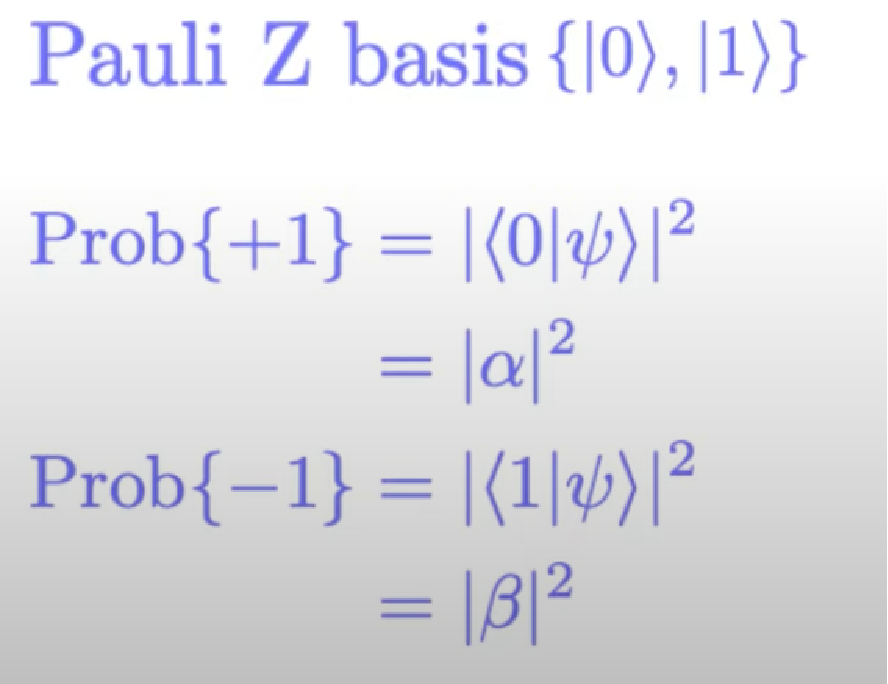
\includegraphics[width=0.5\textwidth]{lesson2/Pauli_z_ex.pdf}
    \label{fig: 1}
    \begin{center}
        \caption{確率:Z軸測定}
    \end{center}
\end{figure}
例えばこれがまあいつも使っているZ軸で計算基底なんですけれども+1の出てくる確率は$0$のベクトルと$\psi$のベクトルの内積でこれを計算すると$\alpha$の絶対値の二乗が出てくる。$-1$の確率が$1$のベクトルなんですけれども$1$のベクトルと$\psi$の内積の絶対値の二乗です。これも$\beta$絶対値の二乗です。これが計算ベクトルで測定してその結果から出てきます。
% Pauli Y example
\begin{figure}[H]
    \centering
    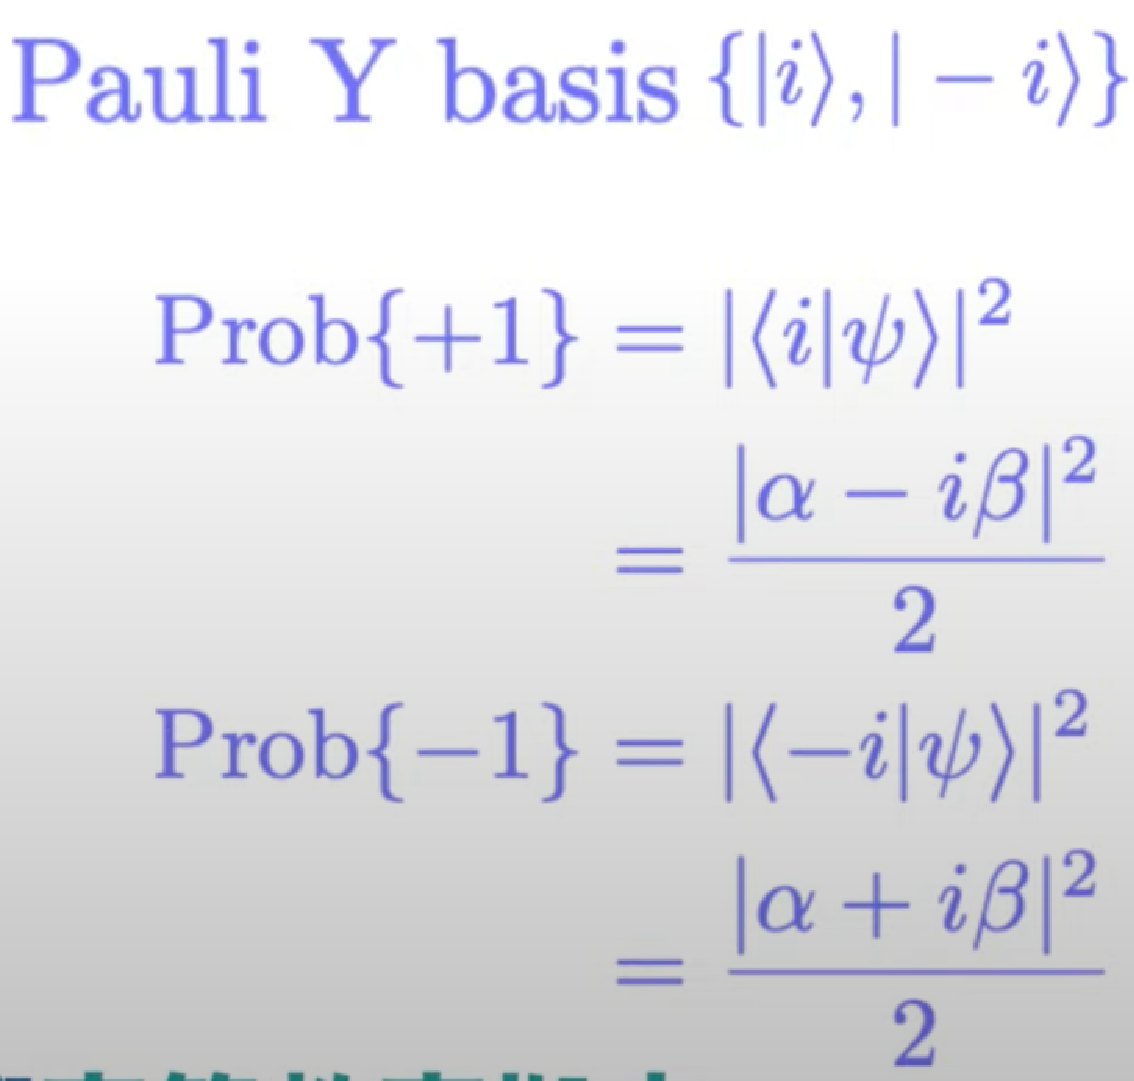
\includegraphics[width=0.5\textwidth]{lesson2/Pauli_y_ex.pdf}
    \label{fig: 1}
    \begin{center}
        \caption{確率:Y軸測定}
    \end{center}
\end{figure}
もう一つの例を挙げると先ほど使っていたYの基底なんですがこのYの基底にすると$i$と$-i$これも同じ風に計算すると$i$と$\psi$の内積を使ってその絶対値をとってそれを二乗にすると出てくるのが$\alpha-i\beta$絶対値の二乗割る2と同様に$-1$もこの表示で出てきます。


\section{確率、期待値、分散}
\subsection{確率}
確率、期待値、分散。Probabilities, expectation, and variance.じゃあちょっと見てみましょう。
先程ステップ3が終わった所なんですけどそれが一つの量子状態を測定したら1回だけの結果が出てきてその状態を破壊して新しい状態が生まれるでしょう。
最後にもっと最初の状態を知りたいなら繰り返さなければいけないと言ってたでしょう。じゃあそれをもうちょっと見てみましょう。
% many copies machine
\begin{figure}[H]
    \centering
    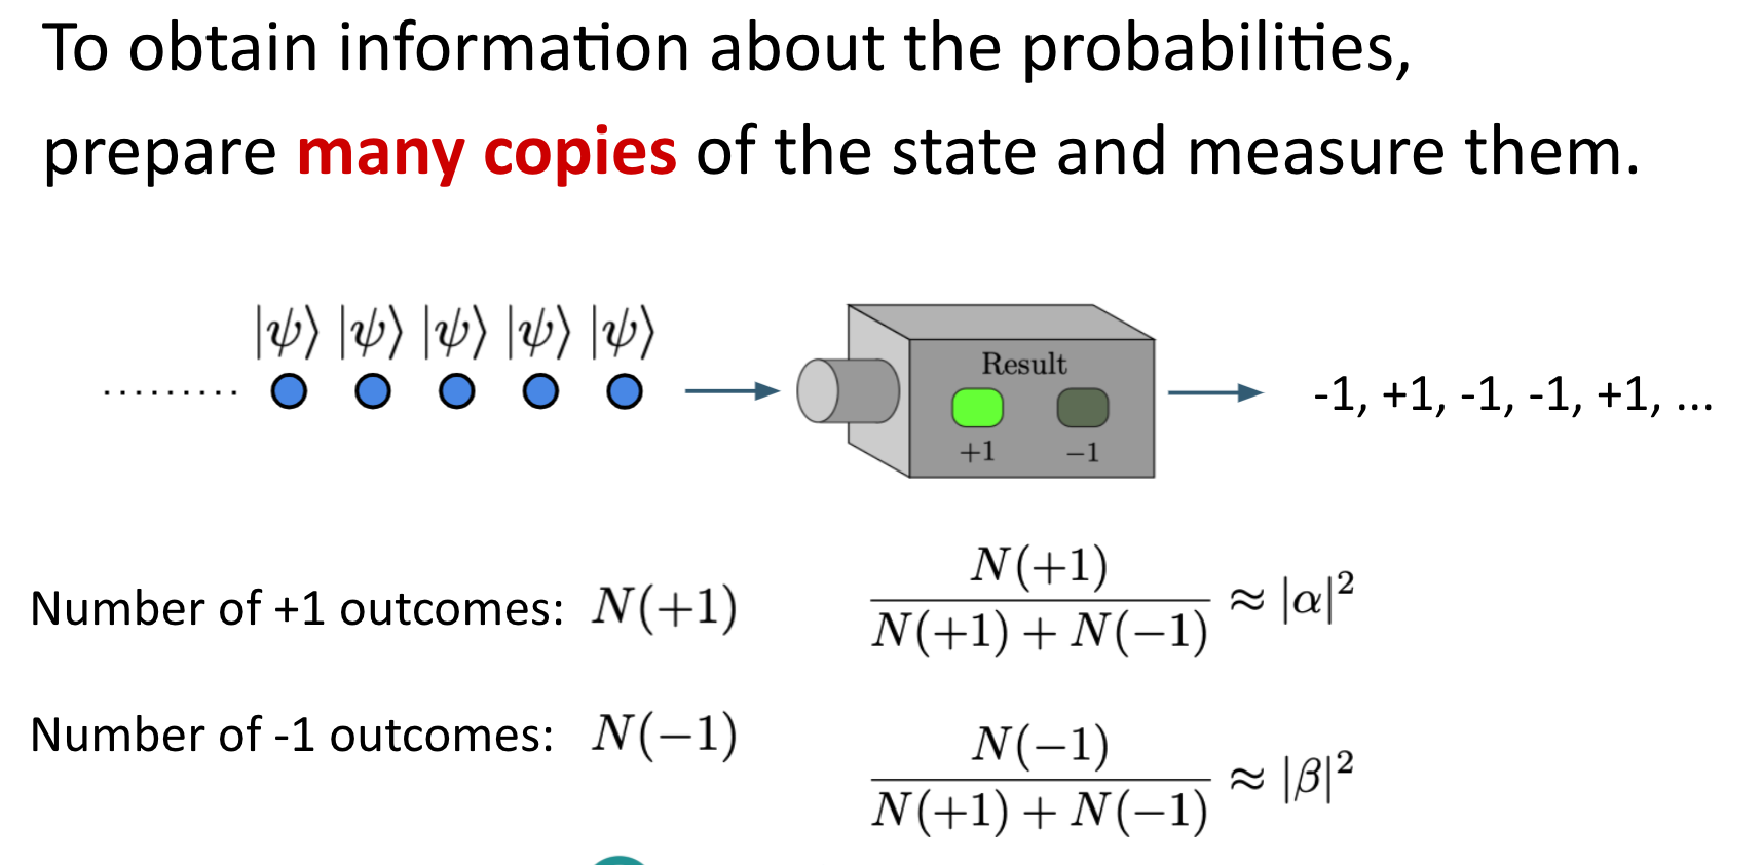
\includegraphics[width=0.5\textwidth]{lesson2/many_copies_machine.pdf}
    \label{fig: 1}
    \begin{center}
        \caption{複数の状態測定}
    \end{center}
\end{figure}
さて、その情報を知りたいなら最初の状態を繰り返していくつかのコピーを作ってそれを連続で測定します。まあそうすると、このように装置が作れるんですが
$\psi$と同じ状態を繰り返し作ってこの機械に入れて出てくることが$-1$, $+1$, $-1$, $+1$の結果が連続で出てくるでしょう。すると$+1$が出てきた数が$N(+1)$と言いますし$-1$が出てきた数が$N(-1)$。これが$\alpha$と$\beta$の情報が計算できるようになります。
\begin{equation}
\begin{aligned}
&\frac{N(+1)}{N(+1)+N(-1)} \approx|\alpha|^{2} \\
&\frac{N(-1)}{N(+1)+N(-1)} \approx|\beta|^{2}
\end{aligned}
\end{equation}

まあこの$N(+1) + N(-1)$はこれが何回このプロセスを繰り返したかを表していると言えるでしょう。それが合計は$\alpha$の絶対値の二乗ぐらいになるでしょう。$N(-1)$を割ると合計が$\beta$の絶対値二乗ぐらいになって-1の出てくる確率になります。

\subsection{期待値}
そうするとこれの期待値はどうなるでしょう。これが基底によります、例えば計算基底、Pauli Z basisの場合の期待値を考えた時Eは確率の授業などで勉強したように:
\begin{equation}
\begin{aligned}
\mathbb{E}[Z] &=\operatorname{Prob}(+1) \cdot(+1)+\operatorname{Prob}(-1) \cdot(-1) \\
&=|\alpha|^{2}-|\beta|^{2}
\end{aligned}
\end{equation}
\textbf{expectation value}(期待値)を例えばこれをDiracの書き方にすると例えばZの基底なのでZをangle bracketの中に入れるとexpectation value(期待値)を示す。

\begin{equation}
\langle Z\rangle=\langle\psi|Z| \psi\rangle
\end{equation}
計算を確認して$\alpha$の絶対値の二乗引く$\beta$の絶対値の二乗になる:
\begin{equation}
\begin{aligned}
\langle Z\rangle &=\left(\begin{array}{ll}
\alpha^{*} & \beta^{*}
\end{array}\right)\left(\begin{array}{cc}
1 & 0 \\
0 & -1
\end{array}\right)\left(\begin{array}{l}
\alpha \\
\beta
\end{array}\right) \\
&=\left(\begin{array}{ll}
\alpha^{*} & \beta^{*}
\end{array}\right)\left(\begin{array}{c}
\alpha \\
-\beta
\end{array}\right) \\
&=|\alpha|^{2}-|\beta|^{2}
\end{aligned}
\end{equation}
これがPauliのZ basis、Z 基底で測定するとこういう結果が出てきます。
\subsection{分散}
もう一つの用語を使うと分散、英語でvarianceと言いますが、出てくる結果が確率的だが最終的には確率が出てきてそのどのぐらいずれている可能性があるかを知りたい場合確率の分布を考えるために分散の概念は必要でしょう。
\begin{equation}
\begin{aligned}
\operatorname{Var}[Z] &=\mathbb{E}\left[Z^{2}\right]-\mathbb{E}[Z]^{2} \\
\mathbb{E}\left[Z^{2}\right] &=\operatorname{Prob}\{+1\} \cdot(+1)^{2}+\operatorname{Prob}\{-1\} \cdot(-1)^{2} \\
&=|\alpha|^{2}+|\beta|^{2}
\end{aligned}
\end{equation}
そうすると\emph{variance}は$Var[Z]$と書いてこれが行列のZの二乗のexpectation value(期待値)引くZの期待値の二乗。もう少し詳しく見ると$\mathbb{E}[Z^2]$の2というのは最初のはbracket(括弧)の中でZの行列の二乗になっており、二つ目では二乗が外なのでZの期待値を測定\emph{してから}二乗している。\textbf{式1.35}が示すように、$\mathbb{E}[Z^2]$は$|\alpha|^2 + |\beta|^2$になります。
%つまりもう少し見るとZの二乗の期待値が+1の確率掛ける-, +1の二乗
% +, -1の確率掛ける-1の二乗なので
% α絶対値の二乗+β絶対値の二乗
% 絶対チヌの事情+データー絶対値の二乗
これは正しく正規化されている場合は$|\alpha|^2 + |\beta|^2 = 1$になるでしょう。

さて最後のこれは時々しか出てきませんがその分散が量子の場合だと\textbf{fluctuation}、 物理学者が使う用語で確率の授業ではvariance(分散)を学んだと思いますが、物理学者はfluctuationという用語を使って\textbf{式1.36}のような書き方もします:
\begin{equation}
\begin{aligned}
(\Delta Z)^{2} & \equiv \operatorname{Var}[Z] \\
&=\left\langle Z^{2}\right\rangle-\langle Z\rangle^{2}
\end{aligned}
\end{equation}

\section{複数の量子ビット}
今まで話たことは例として1量子ビットしか使っていませんでしたがもちろん計算では複数の量子ビットを使いたいですよね。量子通信や量子インターネットに
関しても複数の量子ビットを使いたいでしょう。

まずは複数の古典ビットの場合を復習しましょう。この場合$2^2$の状態は可能ですかね。四つの状態が可能です: $00$, $01$, $10$, $11$。この4つの可能性があります。

量子ビットだったら二つの量子ビットの場合同様です。先程の

$\ket{00}, \ket{01}, \ket{10}, \ket{11}$も同じように出てくるでしょう。この場合これは基底ベクトルだと言えます。そうすると一般的の状態を表示すると、二つの量子ビットの場合このように書きます:
\begin{equation}
|\psi\rangle=\alpha|00\rangle+\beta|01\rangle+\gamma|10\rangle+\delta|11\rangle
\end{equation}
$\alpha$, $\beta$, $\gamma$, $\delta$も正規化が必要です。
$|\alpha|^2 + |\beta|^2$が1つの量子ビットの状態なんですけれども、
これが2量子ビットで4つの状態が可能になるので
これが4つの項を合わせて1になります:
\begin{equation}
|\alpha|^{2}+|\beta|^{2}+|\gamma|^{2}+|\delta|^{2}=1
\end{equation}
$|\gamma|^2$が式から出てくるんですが、測定するとこれが10が出てくる確率になります。4つの確率を合わせて確率全部を計算すると出てくる確率は1なのでこれが正規化と言います。
\begin{equation}
|00\rangle=\left(\begin{array}{l}
1 \\
0 \\
0 \\
0
\end{array}\right),|01\rangle=\left(\begin{array}{l}
0 \\
1 \\
0 \\
0
\end{array}\right),|10\rangle=\left(\begin{array}{l}
0 \\
0 \\
1 \\
0
\end{array}\right),|11\rangle=\left(\begin{array}{l}
0 \\
0 \\
0 \\
1
\end{array}\right)
\end{equation}
そうすると\textbf{式1.39}が4つの基底ベクトル(basis states)になります。
\subsection{ベクトルのテンソル積}

さて\textbf{式1.39}基底はどのように作れるでしょう。
\textbf{Tensor product} テンソルの掛け算で\textbf{式1.40}で表されている記号を使います:
\begin{equation}
|a\rangle \otimes|b\rangle=\left(\begin{array}{l}
a_{1} \\
a_{2}
\end{array}\right) \otimes\left(\begin{array}{l}
b_{1} \\
b_{2}
\end{array}\right) \equiv\left(\begin{array}{l}
a_{1}\left(\begin{array}{l}
b_{1} \\
b_{2}
\end{array}\right) \\
a_{2}\left(\begin{array}{l}
b_{1} \\
b_{2}
\end{array}\right)
\end{array}\right)=\left(\begin{array}{l}
a_{1} b_{1} \\
a_{1} b_{2} \\
a_{2} b_{1} \\
a_{2} b_{2}
\end{array}\right)
\end{equation}
丸の中にばつがある記号です。これが「aのket掛けるbのket掛ける」とも言いますがテンソルの掛け算なので計算の手法が少し違います。テンソルの掛け算と言う場合もありますが、普段は掛け算と省略します。説明のためテンソルを使いたいと思います。

この$
\left(\begin{array}{l}
a_1 \\
a_2
\end{array}\right)$のベクトルと$\left(\begin{array}{l}
b_1 \\
b_2
\end{array}\right)$のベクトルのtensor productを取りたいの\textbf{式1.40}に見えるように解きます。
%で二つ目(後者)のb1 b2のベクトルを
%こっちに置いてそれを掛ける
%前者のベクトルa1 a2と
%a1掛けるb1 b2のベクトル
%下の所でも同じように
%b1 b2のベクトル掛けるそのa2の所で
%前者の所で掛け算になり
%後者のベクトルをそのまま置いて掛けると
%出てくる結果がa1 b1, a1 b2, a2 b1, a2 b2
例として:
\begin{equation}
|0\rangle \otimes|1\rangle=\left(\begin{array}{l}
1 \\
0
\end{array}\right) \otimes\left(\begin{array}{l}
0 \\
1
\end{array}\right)=\left(\begin{array}{l}
0 \\
1 \\
0 \\
0
\end{array}\right)
\end{equation}
$\ket{0}$のベクトルと$\ket{1}$のベクトルをtensor productすると、\textbf{式1.41}で見える通りに解けます。
%この1, 0掛ける0, 1にすると
%まあ1掛けるこの0, 1のベクトル
%この上の半分はそうなり
%下の半分が前者の0掛けるこの0, 1のベクトルで
%これが0, 0になります
もう一つの例として例えば:
\begin{equation}
|1\rangle \otimes|-\rangle=\left(\begin{array}{l}
0 \\
1
\end{array}\right) \otimes \frac{1}{\sqrt{2}}\left(\begin{array}{c}
1 \\
-1
\end{array}\right)=\frac{1}{\sqrt{2}}\left(\begin{array}{c}
0 \\
0 \\
1 \\
-1
\end{array}\right)
\end{equation}
%これが
%1掛ける−の状態
%0, 1のベクトル掛ける√1/2の1, −1のベクトル
%そうするとこの最初の0, 上の0掛ける
%この1, −1のベクトルで上の所は0, 0になるでしょう
%下の所にはこの1掛けるこの1, -1でこれが出てきて
%このconstant(定数)の所には√1/2が出てきます

\subsection{行列のテンソル積}
さてそれがベクトルのtensorの掛け算でしたが、行列でもできます:
\begin{figure}[H]
    \centering
    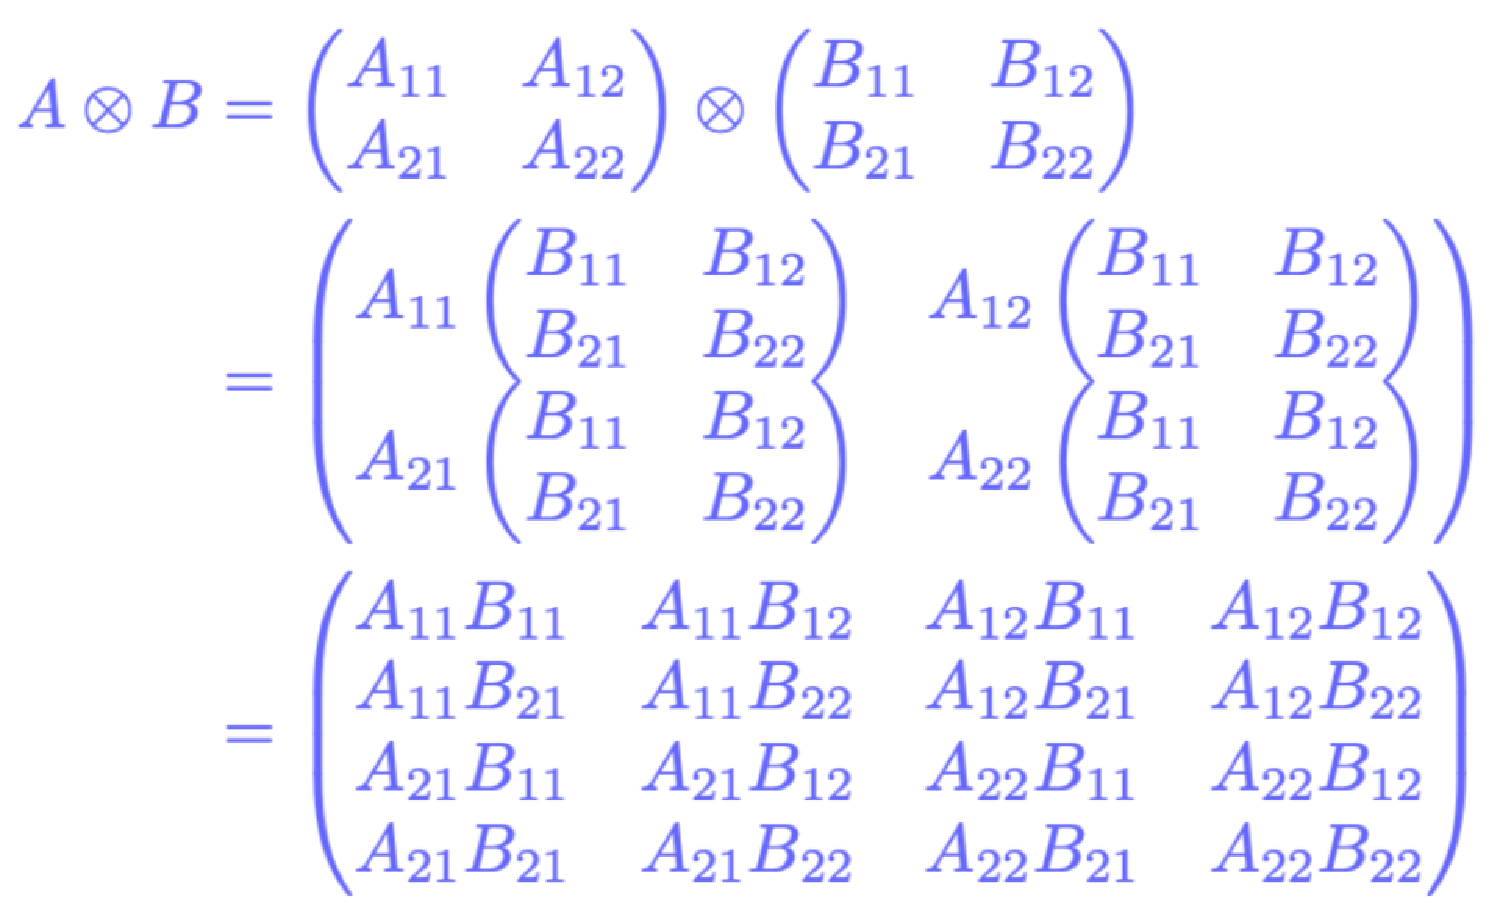
\includegraphics[width=0.8\textwidth]{lesson2/matrix_tensor.pdf}
    \label{fig: 1}
    \begin{center}
        \caption{行列のテンソル}
    \end{center}
\end{figure}
これは$A$の行列と$B$行列の掛け算なんですが、これが普通のベクトルの行列の掛け算ではなくtensorの掛け算なのでtensorproductとしてはこの丸ばつの記号を使います。
\iffalse
%ちょっと拡大するとAの行列はA11 A12 A21 A22
tensor product

0:06:45.608,0:06:50.229
B11 B12  B21 B22で

0:06:50.230,0:06:56.528
すると後者のBの行列を

0:06:56.529,0:07:00.520
そのままこっちに入れて掛けると

0:07:00.837,0:07:10.273
前者のA11でA12 A21 A22の各所に

0:07:10.274,0:07:12.274
Bの行列を掛ける
\fi
そうして全ての組み合わせが出てきて最初の行列が2掛ける2の行列でしたが
結果としては4掛ける4の行列になります。


\begin{equation}
(A \otimes B)|a\rangle \otimes|b\rangle=A|a\rangle \otimes B|b\rangle
\end{equation}
\textbf{式1.43}も\emph{Dirac notation}ですけれども
この場合だったら大文字の$A$が小文字の$a$の状態に演算してますし、この大文字の$B$と小文字の$b$をすると最初の方には$(A \otimes B)|a\rangle \otimes|b\rangle$は右側に等しいです。
\iffalse
かっこa状態tensor product b の状態=

0:08:08.781,0:08:11.571
Aの行列掛けるaの状態掛ける

0:08:11.571,0:08:17.380
tensor product Bの行列掛けるbの状態です
\fi

さて例として見てみましょう。パウリXの演算子を最初の量子ビットだけに作用させましょう:
\begin{equation}
\begin{aligned}
(X \otimes I)|\psi\rangle &=X \otimes I(\alpha|00\rangle+\beta|01\rangle+\gamma|10\rangle+\delta|11\rangle) \\
&=\alpha|10\rangle+\beta|11\rangle+\gamma|00\rangle+\delta|01\rangle
\end{aligned}
\end{equation}
そうすると$(X \otimes I)$は二つ目の量子ビットには何もしないという事を表示しています。
\iffalse
掛けるΨの状態

0:08:43.340,0:08:48.630
それは= X掛けるI

0:08:48.630,0:08:58.572
tensorの掛け算掛けるα00 + β01 + \gamma10 + δ11

0:08:58.572,0:09:08.086
するとα10 +β11 + \gamma00 + δ01
\fi
まあこの掛け算は細かく説明する必要がないと思いますが自分でやってみると良いと思います。でもその最初のX掛けるIを見てみると:
\begin{equation}
(X \otimes I)=\left(\begin{array}{ll}
0 & 1 \\
1 & 0
\end{array}\right) \otimes\left(\begin{array}{ll}
1 & 0 \\
0 & 1
\end{array}\right)=\left(\begin{array}{llll}
0 & 0 & 1 & 0 \\
0 & 0 & 0 & 1 \\
1 & 0 & 0 & 0 \\
0 & 1 & 0 & 0
\end{array}\right)
\end{equation}
左上の部分は全部0になり、右上の部分はこれが$I$になる。左下も$I$になるんですけども右下の所は全部0になります。じゃあ細かいレベルで見ると後者の$\left(\begin{array}{ll}
1 & 0 \\
0 & 1
\end{array}\right)$の行列がありますがもうちょっと拡大(zoom out)して見ると
この形は前者の$\left(\begin{array}{ll}
0 & 1 \\
1 & 0
\end{array}\right)$ の行列と似ているでしょう。この様に掛け算はします。
